\section{Introduction}\label{sec:introduction}

\begin{figure}[htbp]
    \centerline{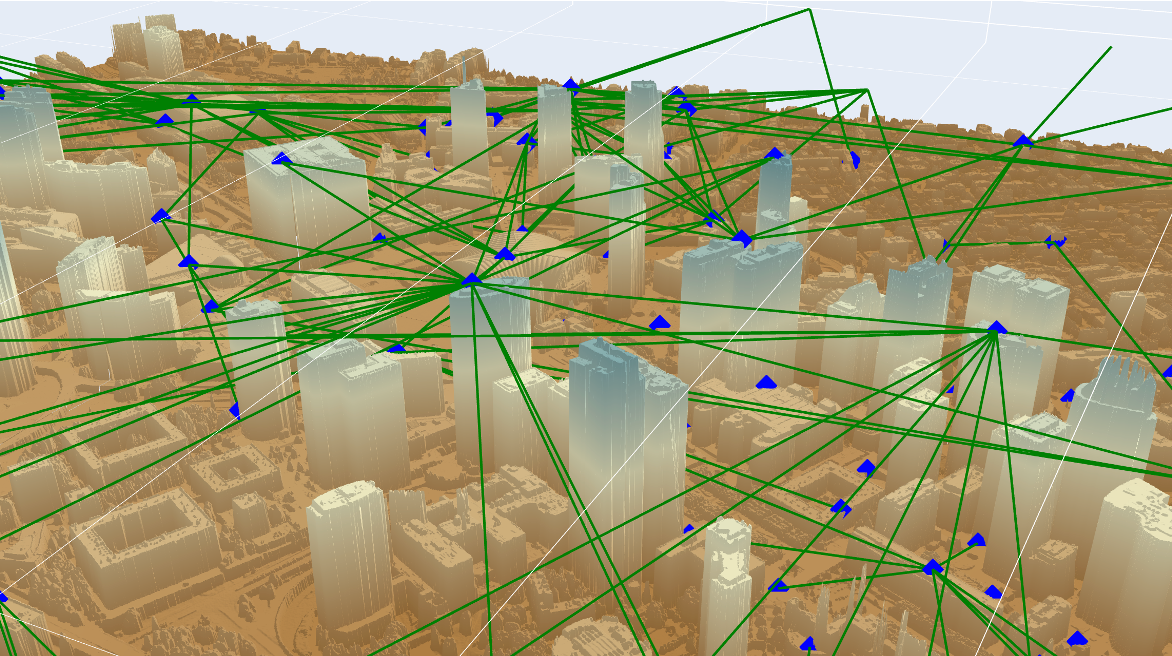
\includegraphics[width=\columnwidth]{figures/scenario}}
    \caption{Clear lines-of-sight for an urban FSO network.}
    \label{fig:scenario}
\end{figure}

Free-Space Optics (FSO) is a technology that uses light beams for wireless point-to-point communication through air.
It offers fiber-like bandwidths without the trenching/leasing costs or spectrum licensing fees typically associated with wired alternatives and radio frequency alternatives, respectively~\cite{urbanfsosurvey}.
While experiments show terabit-speeds over many kilometers on earth~\cite{fastfsozurich, fastfsourban, fastfsojapan} and through the solar system in space~\cite{nasaspace}, the unguided channel limits data rate and link length during weather conditions that scatter and refract the light, such as fog, rain and turbulence~\cite{systematicsurvey}.
Simulations have to focus on the worst-case conditions to guarantee high availability, crucial for consistent QoS and QoE~\cite{outageqoe}.
Relaying traffic at several intermediate hops mitigates the problem by splitting long paths up into shorter ones that withstand adverse conditions better~\cite{relays, hybridfso}.
Urban networks may, as a consequence, due to their dense mesh nature, emerge as a natural fit for highly available FSO networks.
Besides the best-case bandwidths and lack of trenching and spectrum license costs, a mesh FSO deployment comes with several other anticipated advantages.
High redundancy to more hierarchical topologies has the potential to protect against momentary and equipment outages, e.g.,\ from momentary obstructions in the line-of-sight like birds, or power loss of a relay~\cite{fsomeshsurvey}.
The wireless and license-free nature allows for flexible and rapid deployment.
Systems can be ``operative within hours'' and have acted as spontaneous backup links during disasters or irregular events~\cite{urbanfsosurvey}.
In contrast to high upfront costs of laying fiber, an FSO mesh can be deployed gradually, decreasing capital expenditures~\cite{fiberwithoutfiber}.
As average link length shrinks at higher density, we will see that the network benefits from scaling in density, potentially promoting Fixed Wireless Access and reusing the FSO infrastructure for both Cellular Backhaul and Last Mile (``FSO To The Building'').
Removing the wire reduces the risk for an entire class of vulnerabilities, such as excavation accidents, landslides and earthquakes~\cite{fsodigging, fibervulnerability}.

FSO has a research history dating back to 1880~\cite{fsosurveydefault}.
Many of the hard engineering challenges have been ``solved in the past three decades''~\cite{invited}, but some challenges, especially specific to the urban environment, remain: Eye safety regulations vary by country, but may limit transmission power, building sway adds beam alignment complexity, and heat shimmer above hot roofs causes signal scintillation~\cite{urbanfsosurvey, fsobackhaul}.

One of the biggest remaining obstacles for urban FSO, however, originates from the point-to-point nature of FSO links: A line-of-sight must exist between transmitter and receiver~\cite{systematicsurvey}.

\subsection*{Contributions}\label{subsec:contributions}

In this thesis, we develop and implement a method to check individual lines for line-of-sight availability.

Our goal is to analyze the topology of urban networks created purely from verified lines-of-sight.

As link ranges that can be sustained are limited during worst case conditions, we will provide network connectivity metrics over topologies that deploy only links up to a variable maximum length.
From that data, we can derive values that suggest what link ranges need to be supported for various degrees of connectivity in urban FSO networks.
This data can also aid in the judgment which priority needs to be given to the FSO line-of-sight requirement during selection of node locations (for example, as opposed to cellular coverage or cost), or in an extreme case, how well FSO can be retrofitted to existing sites and what role additional mirrors and relays play.

Data rate and capacity simulations are out of the scope of this work, but can build on this work by selecting a set of gateway locations, which connect the FSO network to the internet backbone, and simulating traffic flows from the edge to the gateways.

As a sample dataset for an urban network, we choose an official database of cell sites, simulating a mobile backhaul backbone.
We ran the simulation for 19 million lines in the greater Paris area and find that in a topology of links of up to one kilometer length, 91\% of the considered nodes have at least one line-of-sight.
Moreover, increasing link length beyond around one kilometer has diminishing returns in increased connectivity, but vastly increases options for redundancy and reduces the average hop count between nodes.
At 300 m, a single connected component emerges covering the city of Paris, with 95.8\% of nodes in the region covered by its concave hull connected to the component.

maybe: Short lines (due to worst-case assumption) aid line-of-sight availability.

maybe: Small world: Hop count can be reduced during good conditions